\documentclass[tikz,border=2pt]{standalone}
\usepackage{amsmath,amssymb}
\usepackage{tikz}
\usetikzlibrary{arrows.meta}

\begin{document}
% A mixed integer program with x_1 integer and x_2 continuous: the feasible set is a set of
% vertical segments (integer x_1, any x_2 allowed by the constraints).
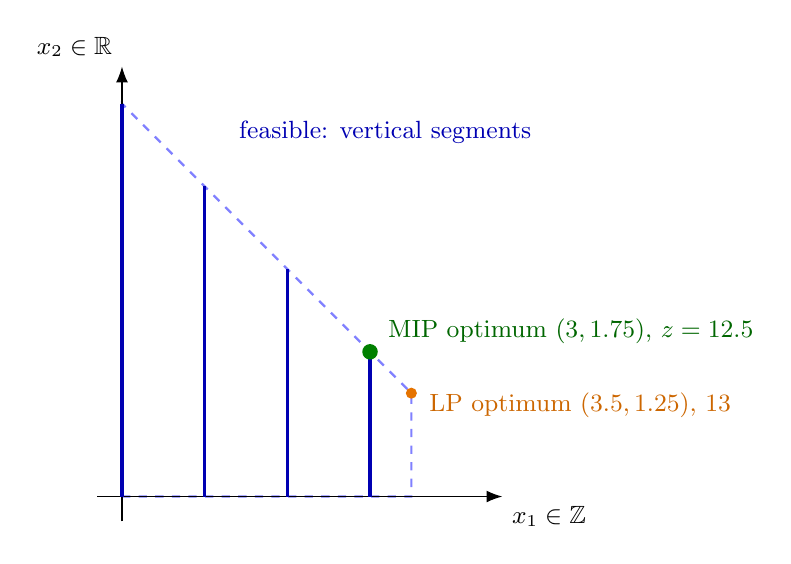
\begin{tikzpicture}[x=1.05cm, y=1.05cm, every node/.style={font=\small}, >={Latex[length=2mm]}]
	\draw[blue!50, thick, dashed] (0,0) -- (3.5,0) -- (3.5,1.25) -- (0,4.75) -- cycle;
	\draw[->] (-0.3,0) -- (4.6,0) node[below right] {$x_1\in\mathbb{Z}$};
	\draw[->] (0,-0.3) -- (0,5.2) node[above left] {$x_2\in\mathbb{R}$};
	\draw[blue!70!black, very thick] (0,0) -- (0,4.75);
	\draw[blue!70!black, very thick] (1,0) -- (1,3.75);
	\draw[blue!70!black, very thick] (2,0) -- (2,2.75);
	\draw[blue!70!black, very thick] (3,0) -- (3,1.75);
	\fill[green!50!black] (3,1.75) circle (2.8pt);
	\node[green!40!black, font=\small, anchor=west] at (3.1,2.0) {MIP optimum $(3,1.75)$, $z=12.5$};
	\fill[orange!90!black] (3.5,1.25) circle (2pt);
	\node[orange!80!black, font=\small, anchor=west] at (3.6,1.1) {LP optimum $(3.5,1.25)$, $13$};
	\node[blue!70!black, font=\small, anchor=west] at (1.3,4.4) {feasible: vertical segments};
	\end{tikzpicture}
\end{document}
